\chapter{Conclusion}
The goal of this thesis was to demonstrate and verify fault detection and
predictive maintenance techniques on the double-acting pneumatic piston
assembly as a case-study object.

\section{Simulation Model}

One of the outcomes from the thesis is a simulation model of the
double-acting pneumatic piston system built based on differential equations
from the pneumatic-mechanical domain, modeled and developed using
Matlab/Simulink software. The simulation model was estimated with
parameters of healthy system behavior. However, there is an option to
reestimate parameters to fault state and simulate the system in a fault
condition. 

Due to the available measured data and significantly nonlinear dynamics of
the system, the simulation model shows good agreement with the measured
data. In contrast to the model built using Simulink/Simscape library, it is
distinctly less computationally expensive while maintaining numerical
stability. These facts are fundamental when parameter estimation is in
progress.

The simulation model was used to experiment with the system's behavior in
different conditions, model fault situations and generate data to design
and develop robust predictive maintenance algorithms. 


\section{Signal-Based PdM}
Another outcome is verifying the possibility of classification and
detection of a fault condition applying predictive maintenance techniques,
using signal-based and model-based methods.
 
The experiments were performed on a dataset measured on a demonstration
device using seven types of sensors.
  
A signal-based method is based on the extraction of useful information
directly from the signal in time-frequency domains. Each sensor required an
individual approach for preprocessing, extracting features, ranking
features and building the classification models. But generally, there is
minimal preprocessing needed to keep the possible helpful information. 

The table \ref{tab:sensors_final} contains the comparison of sensors in 2
categories, accuracy performed in the test dataset and sensor cost. The
graph \ref{fig:sensors_final_bar} visualizes these data.

Surprisingly, all sensors showed an accuracy of more than 75 \%. Microphones
offer excellent performance from a cost/accuracy perspective, and they are
suitable for installation and maintenance.

\begin{figure}[h!]
    \centering
    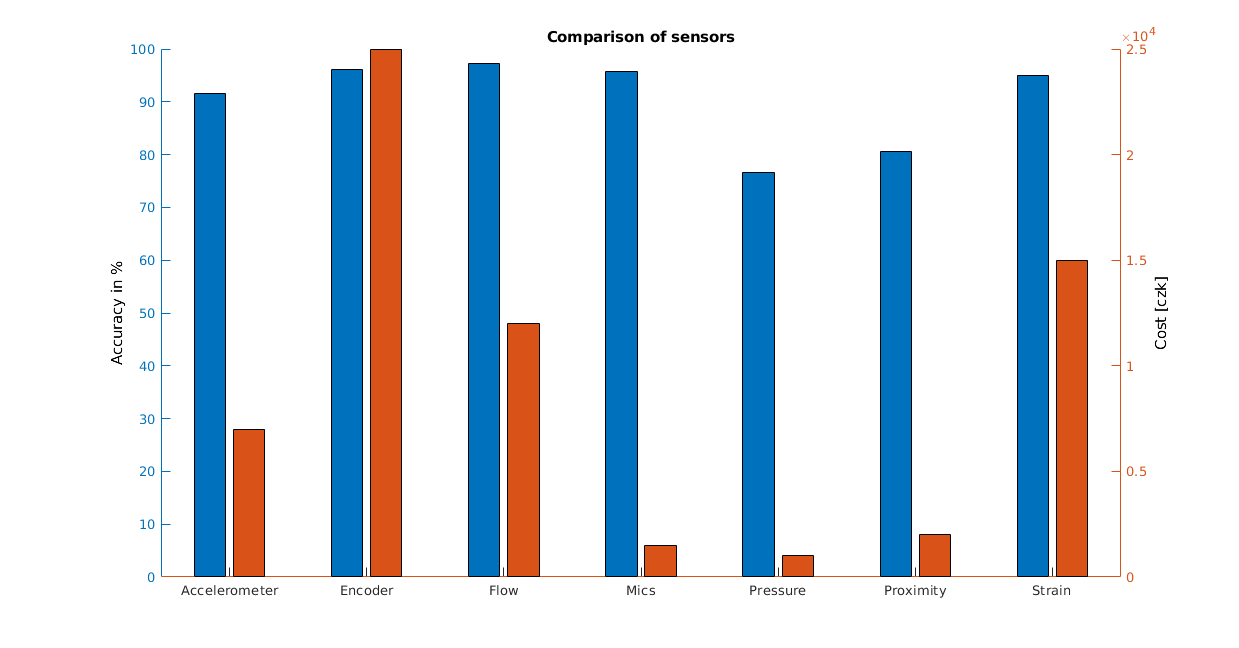
\includegraphics[width=1\textwidth]{sensors_final_bar.png}
    \caption{Comparison of sensors from accuracy/cost perspective}
    \label{fig:sensors_final_bar}
\end{figure}

\begin{table}[h]
    \centering
    \begin{tabular}{|c|c|c|c|c|c|c|c|}
        \hline
        \textbf{Sensor}   & Acc & Encoder & Flow & Mics & Pressure & Proximity & Strain \\
        \hline
        \textbf{Accuracy [\%]} & 91.6 & 96.1 & 97.2 & 95.8 & 76.6 & 80.5 & 95.0 \\
        \hline
        \textbf{Cost [czk]} & 2x 3500 & 25000 & 6000 & 3x 500 & 1000 & 2x 1000 & 15000 \\
        \hline
    \end{tabular}
    \caption{Comparison of sensors from accuracy/cost perspective}
    \label{tab:sensors_final}
\end{table}

\section{Model-Based PdM}

The next part of this thesis was to apply model-based methods and using a
simulation model for predictive maintenance algorithms. These algorithms
are practical when it is hard to extract useful information using a
signal-based method. Or it is suitable in some cases where we understand
the system dynamics and know how to exploit some system variables as
condition indicators.

The use of the method of extraction features in the form of a Nonlinear
system identification model coefficient, specifically with the
Hammerstein-Wiener model, did not give reliable results. Extracted features
have no statistical dependence, and it is impossible to predict fault type
using this method on the measured data from the pneumatic piston as a case
study.

On the other hand, the residual estimation using the simulation model
showed excellent results. The measured position signal was compared with
the signal from the simulation model in normal behavior. This residual
signal was used to classify the fault condition and achieve  99 \% on a
smaller dataset.  But given the results obtained using the signal-based
method, the residual estimation method may seem unnecessary. In this
particular case, from a practical point of view, the improvement of the
result by a few percent does not bring fundamental changes, but the
calculation time increases significantly. 

The possibility of modeling and simulation sensor faults was also verified
using the simulation model. Although it is challenging to collect fault
data from the sensor in real-life conditions, fault data can be generated
from the simulation model and even combined with the primary dataset to
create a synthetical dataset.

\subsection{RUL}
One of the main goals of predictive maintenance is to estimate the
remaining useful life. The original dataset does not contain a record of
historical data that shows degradation behavior. 

A common problem in the maintenance of pneumatic actuators is the leakage
of air from the chamber where the piston is located. This situation was
modeled on the simulation model and generated data were used for RUL
estimation. 

The generated dataset contains 25 simulations with different failure
dynamics. Each simulation includes a different number of cycles depending
on the failure dynamic before the system failure occurs.  Each cycle
contains a 10-second measurement of the system's response.  In the
experiment, a flow signal was chosen as an object of interest. From the
flow signal, the shape factor parameter was calculated and used as a
condition indicator. 

The outcome is that it is possible to estimate the remaining useful life on
generated degradation dataset by using the residual similarity model,
pairwise similarity model and linear degradation model. The prediction
results are satisfying; figure \ref{fig:rul_final} shows the linear
degradation model RUL estimation on the test data.

\begin{figure}[h!]
    \centering
    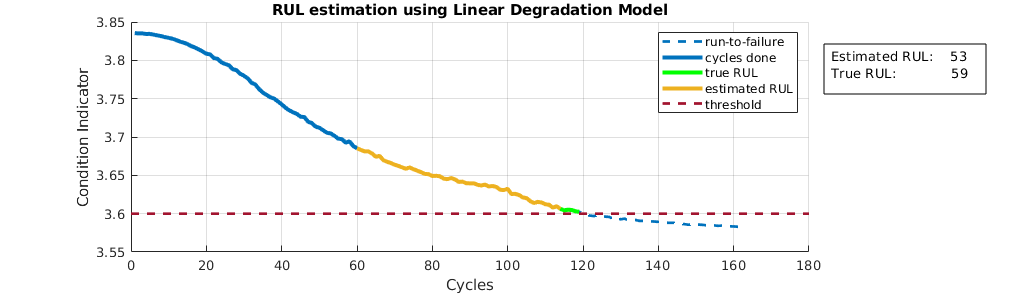
\includegraphics[width=1\textwidth]{rul_final.png}
    \caption{RUL estimation results using linear degradation model}
    \label{fig:rul_final}
\end{figure}

\section{Further Development}
As a further development, it would be appropriate to estimate the modeled
system parameters piecewise to improve the results, emphasizing the
characteristics of throttle valves and dampers with adjustments. 

Perform air leak fault condition measurements and collect historical
degradation data from a real pneumatic piston. Subsequently, evaluate the
dynamics of the failure caused by the air leak. Verify the possibility of
estimating the remaining useful life using a flow sensor. It could be an
interesting case study to verify a possibility of RUL estimation using
microphones. If the performance of the available sensors is deficient, the
pressure measurements in the chamber can be performed. The pressure in the
chamber is directly dependent on the air leakage from the chamber, as
presented in equation \ref{eq:p_B_rul}. An example of pressure changes from the
simulation model is shown in figure \ref{fig:pressure_air_leak}.

